\section{Semi-Implicit Method for Pressure Linked Equations (SIMPLE)}
\label{sec:simple}

After having presented the \acrshort{scgs} algorithm, we will now discuss the \acrfull{simple} method.

The \acrshort{simple} algorithm has been proposed by Patankar and Spalding in 1972 \cite{Patankar1972ACP} and is one of the most used algorithms for solving the Navier-Stokes equations in the field of CFD.

With respect to the coupled approach of the \acrshort{scgs} method, the \acrshort{simple} method decouples the momentum and continuity equations, solving them sequentially.
This approach makes also easier to possibly add more equations to the system, such as the energy equation or the turbulence model, given that would be solved independently of the momentum and continuity equations.

Many of the concepts discussed for the \acrshort{scgs} methods, such as variable correction (Section \ref{subsec:variable_correction_concept}) or the residual (Section \ref{subsec:residual_concept}), or again the Guass-Seide iterative method (Section \ref{subsec:gauss_seidel_iterative_method}), are still valid and we will report in following just their application to the \acrshort{simple} algorithm without repeating the core idea behind them.



The major and fundamental difference between the \acrshort{scgs} and the \acrshort{simple} methods is in the way the equation are coupled together and solved.
In the \acrshort{scgs} method, we have seen in Section \ref{subsec:equations_coupling} and Section \ref{subsec:vanka_approach} that the momentum and continuity equations are coupled together and solved simultaneously.
In the \acrshort{simple} method, instead, the momentum and continuity equations are decoupled and solved sequentially.


\subsection{Derivation of the pressure correction equation}

As we have said in the introduction, the \acrshort{simple} method decouples the momentum and continuity equations, solving them sequentially.
The system of equations is now coupled through the pressure correction term, which can be computed from the residuals of the continuity equation.

In the following, we will derive the pressure correction equation starting from the discretized momentum and continuity equations.

Considering of applying correction to every velocity and pressure term, we obtain the following equations:

\begin{gather}
    (A_P^u)_{i-1,j} (u_{i-1,j}^* + u_{i-1,j}') = \sum_{nb} (A_{nb}^u)_{i-1,j} (u_{nb}^* + u_{nb}')_{i-1,j} + ((p_{i-1,j}^* + p_{i-1,j}') - (p_{i,j}^* + p_{i,j}')) \Delta y \\
    (A_P^u)_{i,j}   (u_{i,j}  ^* + u_{i,j}')   = \sum_{nb} (A_{nb}^u)_{i,j}   (u_{nb}^* + u_{nb}')_{i,j}   + ((p_{i,j}^*   + p_{i,j}') - (p_{i+1,j}^* + p_{i+1,j}')) \Delta y   \\
    (A_P^v)_{i,j-1} (v_{i,j-1}^* + v_{i,j-1}') = \sum_{nb} (A_{nb}^v)_{i,j-1} (v_{nb}^* + v_{nb}')_{i,j-1} + ((p_{i,j-1}^* + p_{i,j-1}') - (p_{i,j}^* + p_{i,j}')) \Delta x \\
    (A_P^v)_{i,j}   (v_{i,j}  ^* + v_{i,j}')   = \sum_{nb} (A_{nb}^v)_{i,j}   (v_{nb}^* + v_{nb}')_{i,j}   + ((p_{i,j}^*   + p_{i,j}') - (p_{i,j+1}^* + p_{i,j+1}')) \Delta x   \\
    ((u_{i,j}^* + u_{i,j}') - (u_{i-1,j}^* + u_{i-1,j}')) \Delta y + ((v_{i,j}^* + v_{i,j}') - (v_{i,j-1}^* + v_{i,j-1}')) \Delta x = 0 \label{eq:SIMPLE_continuity_equation}
\end{gather}

Supposing now to be at the converged solution, and so when the correction terms are approximately zero, we subtract the system of converged equations from the above system, obtaining the following equations:

\begin{gather}
    (A_P^u)_{i-1,j} (u_{i-1,j}') = \sum_{nb} (A_{nb}^u)_{i-1,j} (u_{nb}')_{i-1,j} + ((p_{i-1,j}') - (p_{i,j}')) \Delta y + R^u_{i-1,j} \\
    (A_P^u)_{i,j}   (u_{i,j}')   = \sum_{nb} (A_{nb}^u)_{i,j}   (u_{nb}')_{i,j}   + ((p_{i,j}') - (p_{i+1,j}')) \Delta y + R^u_{i,j}   \\
    (A_P^v)_{i,j-1} (v_{i,j-1}') = \sum_{nb} (A_{nb}^v)_{i,j-1} (v_{nb}')_{i,j-1} + ((p_{i,j-1}') - (p_{i,j}')) \Delta x + R^v_{i,j-1} \\
    (A_P^v)_{i,j}   (v_{i,j}')   = \sum_{nb} (A_{nb}^v)_{i,j}   (v_{nb}')_{i,j}   + ((p_{i,j}') - (p_{i,j+1}')) \Delta x + R^v_{i,j}   \\
    (u_{i,j}' - u_{i-1,j}') \Delta y + (v_{i,j}' - v_{i,j-1}') \Delta x = R^c_{i,j}
\end{gather}

Moreover, we can neglect the residual terms $R^u$ and $R^v$, and the correction terms $u'_{nb}$ and $v'_{nb}$, given that at the convergence of the solution they are approximately zero.

\begin{gather}
    (A_P^u)_{i-1,j} (u_{i-1,j}') = ((p_{i-1,j}') - (p_{i,j}')) \Delta y \\
    (A_P^u)_{i,j}   (u_{i,j}')   = ((p_{i,j}') - (p_{i+1,j}')) \Delta y \\
    (A_P^v)_{i,j-1} (v_{i,j-1}') = ((p_{i,j-1}') - (p_{i,j}')) \Delta x \\
    (A_P^v)_{i,j}   (v_{i,j}')   = ((p_{i,j}') - (p_{i,j+1}')) \Delta x \\
    (u_{i,j}' - u_{i-1,j}') \Delta y + (v_{i,j}' - v_{i,j-1}') \Delta x = R^c_{i,j}
\end{gather}

By doing so, we can now rearrange the equations so to write every velocity correction as a function of the pressure correction term:

\begin{gather}
    u_{i,j}' = \frac{\Delta y}{(A_P^u)_{i,j}} (p_{i,j}' - p_{i+1,j}') \\
    u_{i-1,j}' = \frac{\Delta y}{(A_P^u)_{i-1,j}} (p_{i-1,j}' - p_{i,j}') \\
    v_{i,j}' = \frac{\Delta x}{(A_P^v)_{i,j}} (p_{i,j}' - p_{i,j+1}') \\
    v_{i,j-1}' = \frac{\Delta x}{(A_P^v)_{i,j-1}} (p_{i,j-1}' - p_{i,j}')
\end{gather}

Similarly, we can rearrange the continuity equation as a function of the pressure correction term only:

\begin{align}
     & \left(\frac{\Delta y}{(A_P^u)_{i,j}} (p_{i,j}' - p_{i+1,j}') - \frac{\Delta y}{(A_P^u)_{i-1,j}} (p_{i-1,j}' - p_{i,j}')\right) \Delta y + \dots       \\
     & + \left(\frac{\Delta x}{(A_P^v)_{i,j}} (p_{i,j}' - p_{i,j+1}') - \frac{\Delta x}{(A_P^v)_{i,j-1}} (p_{i,j-1}' - p_{i,j}')\right) \Delta x = R^c_{i,j}
\end{align}

We can now explicitly write the pressure coefficients by rearranging the equations above:

\begin{align}
    (A_E^p)_{i,j} & = \frac{(\Delta y)^2}{(A_P^u)_{i,j}}                            \\
    (A_W^p)_{i,j} & = \frac{(\Delta y)^2}{(A_P^u)_{i-1,j}}                          \\
    (A_N^p)_{i,j} & = \frac{(\Delta x)^2}{(A_P^v)_{i,j}}                            \\
    (A_S^p)_{i,j} & = \frac{(\Delta x)^2}{(A_P^v)_{i,j-1}}                          \\
    (A_P^p)_{i,j} & = (A_E^p)_{i,j} + (A_W^p)_{i,j} + (A_N^p)_{i,j} + (A_S^p)_{i,j}
    \label{eq:SIMPLE_pressure_coefficients}
\end{align}

The pressure correction equation then becomes:

\begin{equation}
    (A_P^p)_{i,j} p_{i,j}' = \sum_{nb} (A_{nb}^p)_{i,j} p_{nb}' + R^c_{i,j}
\end{equation}


\subsection{Algorithm}

As we have said at the beginning of this section, the \acrshort{simple} method decouples the momentum and continuity equations, solving them sequentially.

\subsubsection{Initialization}

At first, all the states ($u*$, $v*$, $p*$) are initialized to zero.

\subsubsection{$u$ Momentum equation}

\paragraph{Compute the coefficients}

The coefficients $A_P^u$, $A_{nb}^u$ are computed for the entire domain based on the convection and diffusion schemes adopted (see Section \ref{subsec:final_coefficients}).

\paragraph{Apply the boundary conditions}

The boundary conditions for the velocity field are applied. See section \ref{subsec:SIMPLE_boundary_conditions} for more details.

\paragraph{Application of the Gauss-Seidel method}

In order to compute the pressure correction, we need at first to compute the continuity residual $R^c_{i,j}$.
To do so, we need to obtain a first approximation of the velocity field by solving the momentum equations.

Here, we apply iteratively the Gauss-Seidel method to solve the momentum equations for all the cells in the domain.

\begin{equation}
    u_{i,j}^* = \alpha_u \left( \frac{\sum_{nb} (A_{nb}^u)_{i,j} u_{nb}^* - (p_{i,j}^* - p_{i+1,j}^*) \Delta y}{(A_P^u)_{i,j}} \right) + (1 - \alpha_u) u_{i,j}^*
\end{equation}


\subsection{$v$ Momentum equation}

\paragraph{Compute the coefficients}

The coefficients $A_P^v$, $A_{nb}^v$ are computed for the entire domain based on the convection and diffusion schemes adopted (see Section \ref{subsec:final_coefficients}).

\paragraph{Apply the boundary conditions}

The boundary conditions for the velocity field are applied. See section \ref{subsec:SIMPLE_boundary_conditions} for more details.

\paragraph{Application of the Gauss-Seidel method}

Similarly to what we have done for the $u$ momentum equation, we now have to apply iteratively the Gauss-Seidel method to solve the momentum equations for all the cells in the domain.

\begin{equation}
    v_{i,j}^* = \alpha_v \left( \frac{\sum_{nb} (A_{nb}^v)_{i,j} v_{nb}^* - (p_{i,j}^* - p_{i,j+1}^*) \Delta x}{(A_P^v)_{i,j}} \right) + (1 - \alpha_v) v_{i,j}^*
\end{equation}


\subsection{Pressure correction}

\paragraph{Compute the coefficients}

The coefficients $A_P^p$, $A_{nb}^p$ are computed for the entire domain based on $A_P^u$ and $A_P^v$. See Equations \ref{eq:SIMPLE_pressure_coefficients} for more details.

\paragraph{Apply the boundary conditions}

The boundary conditions for the pressure field are applied. See section \ref{subsec:SIMPLE_boundary_conditions} for more details.

\paragraph{Compute the continuity residual}

The continuity residual $R^c_{i,j}$ is computed for all the cells in the domain based on the solution of the momentum equations obtained during the Gauss-Seidel iterations.

\begin{equation}
    R^c_{i,j} = -((u_{i,j}^* - u_{i-1,j}^*) \Delta y + (v_{i,j}^* - v_{i,j-1}^*) \Delta x)
\end{equation}

\paragraph{Application of the Gauss-Seidel method}

As we have done for the momentum equations, we now apply iteratively the Gauss-Seidel method to solve the pressure correction equation for all the cells in the domain.

\begin{equation}
    p_{i,j}' = \frac{\sum_{nb} (A_{nb}^p)_{i,j} p_{nb}' + R^c_{i,j}}{(A_P^p)_{i,j}}
\end{equation}


\subsubsection{Update the velocity and pressure fields}

Finally, based on the pressure correction term, we can update the velocity and pressure fields.

\begin{align}
    p_{i,j}^* & = p_{i,j}^* + \alpha_p p_{i,j}'                                               \\
    u_{i,j}^* & = u_{i,j}^* - \alpha_u \frac{\Delta y}{(A_P^u)_{i,j}} (p_{i,j}' - p_{i+1,j}') \\
    v_{i,j}^* & = v_{i,j}^* - \alpha_v \frac{\Delta x}{(A_P^v)_{i,j}} (p_{i,j}' - p_{i,j+1}')
\end{align}


\subsubsection{Convergence criterion}

The convergence criterion for the \acrshort{simple} algorithm is based on the residuals of the continuity and pressure correction equations.

In particular, the convergence criterion is satisfied when the maximum value of the sum of all the residuals is below a certain threshold, which is:

\begin{equation}
    \max \left(\sum_{i,j} |R^u_{i,j}|, \sum_{i,j} |R^v_{i,j}|, \sum_{i,j} |R^{pp}_{i,j}| \right) < \epsilon
\end{equation}

Until the convergence criterion is not satisfied, the algorithm will continue to iterate.



\subsection{Boundary conditions for Lid-Driven Cavity problem}
\label{subsec:SIMPLE_boundary_conditions}

The boundary conditions for the \acrshort{simple} algorithm are based on the same idea of No-Slip and No-Penetration conditions as for the \acrshort{scgs} algorithm.
Their implementation, however, is slightly different.

As we have done for the \acrshort{scgs} algorithm, we will consider the Lid-Driven Cavity problem to explain how the boundary conditions are applied.
In particular, we can consider the top-left corner of the domain as represented in Figure \ref{fig:SIMPLE_domain}.

\begin{figure}[H]
    \centering
    \def\nCV{2}
    \def\dX{3cm}
    \def\dY{3cm}

    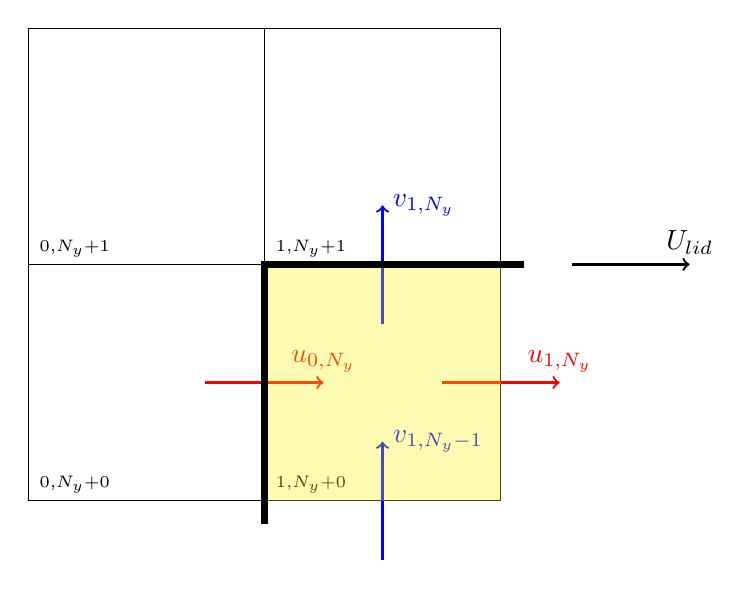
\begin{tikzpicture}

        \foreach \n in {0,1,...,\nCV}
            {
                \draw (0, \n*\dY) -- (\nCV*\dX, \n*\dY);
                \draw (\n*\dX, 0) -- (\n*\dX, \nCV*\dY);
            }

        \foreach \y in {0,1,...,\the\numexpr\nCV-1\relax}
            {
                \foreach \x in {0,1,...,\the\numexpr\nCV-1\relax}
                    {
                        \node[font=\small] at (\x*\dX+\dX/5, \y*\dY+\dY/15) {$_{\x, N_y+\y}$};
                    }
            }

        \draw[thick, blue, ->] (3/2*\dX, 1/2*\dY)++(0,  \dY/4) -- ++(0, \dY/2) node[pos=1, right] {$v_{1,N_y}$};
        \draw[thick, blue, ->] (3/2*\dX, 1/2*\dY)++(0, -\dY/2-\dY/4) -- ++(0, \dY/2) node[pos=1, right] {$v_{1,N_y-1}$};
        \draw[thick, red, ->] (3/2*\dX, 1/2*\dY)++(\dX/4, 0) -- ++(\dX/2, 0) node[pos=1, above] {$u_{1,N_y}$};
        \draw[thick, red, ->] (3/2*\dX, 1/2*\dY)++(-\dX/2-\dX/4, 0) -- ++(\dX/2, 0) node[pos=1, above] {$u_{0,N_y}$};

        \fill[yellow, opacity=0.3] (\dX, 0) rectangle (2*\dX, \dY);

        \draw[line width=1mm] (\dX, -\dY/10) -- (\dX, \dY) -- (2*\dX+\dX/10, \dY);
        \draw[thick, ->] (2*\dX +\dX/10, \dY) ++(\dX/5, 0) -- ++(\dX/2, 0) node[pos=1, above] {$U_{lid}$};

    \end{tikzpicture}
    \caption{Boundary conditions for the cell $(1, N_y)$}
    \label{fig:SIMPLE_domain}
\end{figure}

Considering Figure \ref{fig:SIMPLE_domain}, and in particular the cell $(1, N_y)$, we can write the boundary conditions for the velocity field as follows:

\begin{align}
    u_{0, N_y}   & = 0       \\
    u_{1, N_y}   & = U_{lid} \\
    v_{1, N_y-1} & = 0       \\
    v_{1, N_y}   & = 0
    \label{eq:SIMPLE_velocity_boundary_conditions}
\end{align}

The boundary conditions for the pressure field are instead:

\begin{align}
    p_{0, N_y} & = p_{1, N_y} \\
    p_{1, N_y} & = p_{0, N_y}
    \label{eq:SIMPLE_pressure_boundary_conditions}
\end{align}

Similar consideration can be done for the other boundaries of the domain.


\subsubsection{Application of the boundary conditions}

When it comes to apply the boundary conditions for the \acrshort{simple} algorithm, we need to either modify directly the velocity fields or, for pressure, we need to modify the coefficients of the pressure correction equation.

\paragraph{$u$ Boundary conditions}

In order to satisfy Equations \ref{eq:SIMPLE_velocity_boundary_conditions}, for the $u$ velocity field we can directly modify the velocity field as:

\begin{align}
    u_{0, N_y} & = 0                                                                                     \\
    U_{lid}    & = \frac{u_{1, N_y} + u_{1, N_y+1}}{2} \rightarrow u_{1, N_y+1} = 2 U_{lid} - u_{1, N_y}
\end{align}

\paragraph{$v$ Boundary conditions}

Similarly to what we have done for the $u$ velocity field, we can directly modify the velocity field as:

\begin{align}
    v_{1, N_y} & = 0                                                                               \\
    0          & = \frac{v_{1, N_y-1} + v_{0, N_y-1}}{2} \rightarrow v_{0, N_y-1} = - v_{1, N_y-1}
\end{align}

\paragraph{Pressure Boundary conditions}

For the pressure field, we need to modify the coefficients of the pressure correction equation.

\begin{align}
    (A_W^p)_{1, N_y} & = 0 \\
    (A_N^p)_{1, N_y} & = 0
\end{align}

By doing so, the pressure correction equation for the cell $(1, N_y)$ becomes:

\begin{equation}
    (A_P^p)_{1, N_y} p_{1, N_y}' = ((A_E^p)_{1, N_y} + (A_S^p)_{1, N_y}) p_{1, N_y}' = (A_E^p)_{1, N_y} p_{2, N_y}' + (A_S^p)_{1, N_y} p_{1, N_y-1}' + R^c_{1, N_y}
\end{equation}

